\chapter{Analisis Persoalan dan Rancangan Solusi}

Tujuan utama penulisan bab ini adalah untuk menguraikan rencana penyelesaian masalah tugas akhir sebelum dieksekusi. Bagian ini akan memaparkan proses analisis masalah hingga menjadi solusi.

\subsection{Analisis Permasalahan}
\label{sec:analisis-permasalahan}

Pada lingkungan \textit{IoT}, berbagai perangkat terhubung memainkan peran penting dalam mengumpulkan dan memproses data dari lingkungan sekitarnya. Perangkat ini sering kali terbatas sumber daya, memiliki kapasitas pemrosesan, memori, dan penyimpanan yang minim. Meskipun begitu, ada kebutuhan yang meningkat untuk mengerahkan logika aplikasi yang kompleks secara langsung ke perangkat-perangkat ini untuk meningkatkan efisiensi, mengurangi latensi, dan mendukung operasi \textit{offline} atau semi-\textit{offline}. Masalah utama yang muncul adalah bagaimana secara efisien mengelola dan mengerahkan komponen aplikasi pada skala besar dalam lingkungan yang sangat heterogen dan terbatas sumber daya.

Berdasarkan latar belakang yang telah diuraikan pada \textbf{Bagian \ref{sec:latar-belakang}}, masalah ini dapat diselesaikan dengan menggunakan \textit{remote deployment}. Namun, proses pembuatan layanan agar dapat melakukan \textit{remote deplotment} untuk perangkat yang heterogen menjadi hal yang cukup sulit, perlu dibuat sebuah sistem yang mengatur seluruh proses agar menjadi konsisten dan \textit{well documented}. Sistem ini juga bermanfaat untuk pengguna yang ingin mencoba mengembangkan sistem untuk menambah berbagai fitur kedepannya. Standar ini akan terdiri dari model \textit{deployment} serta layanan orkestrasi untuk membantu proses pengelolaan. Layanan orkestrasi, berperan cukup penting dalam sistem, dengan adanya layanan ini proses pengelolaan perangkat yang heterogen menjadi cukup mudah untuk dilakukan. Selain layanan orkestrasi, \textit{deployment plan} model pun perlu memiliki standar agar dapat digunakan oleh \textit{client} atau \textit{developer}.

Sistem dibuat dengan menyediakan infrastruktur yang berorientasi layanan untuk pengerahan komponen aplikasi yang elastis pada perangkat yang memiliki sumber daya yang terbatas pada IoT dengan skala besar. Sistem harus memiliki dukungan untuk melakukan \textit{deployment} berbasis push, serta mengetahui kondisi dari setiap perangkat. Sistem yang dibuat perlu memiliki cara untuk membuat sebuah resep deployment yang terdiri dari beberapa komponen iot serta
pemrosesan paket aplikasi yang disesuaikan dengan platform perangkat, dan mekanisme skalabilitas untuk mengelola penyebaran ke jumlah perangkat yang besar dengan efisien.

Untuk membuat implementasi dari sistem \textit{remote deployment}, terdapat beberapa rintangan yang perlu diatasi. Rintangan tersebut, dapat dirumuskan ke dalam poin-poin sebagai berikut.

\begin{enumerate}
  \item Kondisi saat ini belum banyak sistem \textit{IoT} yang dibuat dan diorkestrasi menggunakan \textit{kubernetes}
  \item Belum ada \textit{deployment plan} yang dapat mendefinisikan proses \textit{deployment} serta agar \textit{remote deployment} dapat diorkestrasi  dengan menggunakan \textit{kubernetes}
  \item Sistem dapat berjalan meskipun dalam kondisi buruk.
  \item Sistem dapat mengetahui kondisi dari masing masing perangkat serta proses \textit{deployment} yang sedang berjalan.
  \item Sistem dapat melakukan deployment dengan metode \textit{push}, sehingga setiap perangkat yang terhubung akan melakukan proses pembaruan secara otomatis.
\end{enumerate}


\section{Analisis Solusi}

Berdasarkan analisis permasalahan pada \ref{sec:analisis-permasalahan} serta studi literatur, Terdapat tiga alternatif solusi untuk mengatasi permasalahan tesrebut.
Mengembangkan sebuah sistem yang memiliki \textit{reliability} dan \textit{observability} yang baik dengan skalabilitas yang tinggi dengan menggunakan kubernetes dengan \textit{service mesh}. Membuat sistem dengan \textit{reliability} yang baik  menggunakan protokol \textit{MQTT}, serta peningkatan layanan internet pada setiap lingkungan disekitar perangkat \textit{IoT}.

\subsection{Perangkat IoT dibekali dengan Internet yang baik}
Salah satu cara untuk mengatasi masalah ini yaitu dengan menaruh internet yang baik disekitar perangkat \textit{IoT}. Dengan adanya hal ini, proses \textit{reliability} akan tercapai serta sistem juga akan memiliki latensi yang rendah. Namun, cara ini tidak optimal dan membutuhkan biaya yang cukup mahal.

Perlu ditempatkan internet yang baik di sekitar perangkat \textit{IoT} memerlukan biaya yang cukup banyak dan cara ini sepenuhnya bergantung pada kualitas \textit{internet service provider} yang digunakan. Apabila \textit{ISP} sedang mengalami penurunan kualitas dan membuat jaringan menjadi buruk maka cara ini sistem akan langsung \textit{unreliable}.

\subsection{Membuat sistem menggunakan protokol MQTT untuk melakukan pertukaran data}
Akan dibuat suatu sistem yang dapat berkomunkasi menggunakan protokol \textit{MQTT}. Sistem ini terdiri dua komponen, \textit{client} dan \textit{broker}. MQTT \textit{client} berfungsi untuk melkukan \textit{subscribe} ataupun \textit{publish} data ke MQTT \textit{broker}. MQTT \textit{broker} sendiri akan menyimpan data yang dikirim oleh sensor ataupun perangkat \textit{IoT} lainnya (publish) dan memiliki reliability yang sangat tinggi sehingga seberapa burukpun jaringannya akan tetap dapat diterima dengan baik \parencite{mqtt}.

\subsection{Membuat \textit{Smart Home System} berbasis Service Mesh dengan kubernetes}
Untuk membuat suatu sistem yang memenuhi dan menjawab permasalahan yang telah diangkat sebelumnya, dapat dibuat suatu sistem menggunakan kubernetes berbasis service mesh





% \subsection{Arsitektur standar untuk \textit{deployment} pada KubeEdge}
% Untuk membuat arsitektur pada KubeEdge perlu memerlukan beberapa konsiderasi terutama pada bagian \textit{EdgeCore}. Secara konsep arsitektur pada KubeEdge tidak jauh berbeda dari kubernetes pada umumnya, namun terdapat perbedaan cara berkomunkasi dari bagian \textit{cloud} dengan \textit{edge} serta komunikasi antar perangkat \textit{IoT} pada \textit{Edge} yang menggunakan MQTT. Dengan melakukan percobaan \textit{deploy} dengan KubeEdge dan melihat referensi pada \ref{sec:riset-terkait} proses standardiasi arsitektur akan mudah untuk dilakukan

% \subsection{Meningkatkan \textit{device discovery} pada layanan}
% Dengan melakukan integrasi dengan \textit{Service Mesh} proses \textit{device discovery} menjadi lebih mudah untuk dilakukan karena untuk setiap aplikasi yang di\textit{deploy} menggunakan KubeEdge, akan ditambah sebuah \textit{sidecar proxy} untuk proses penerimaan maupun pengiriman \textit{request}. Dengan adanya \textit{sidecar proxy} proses \textit{device discovery} menjadi lebih mudah untuk dilakukan.

% \subsection{Menurunkan \textit{low latency} pada layanan}
% Tantangan utama pada aplikasi yang terintegrasi dengan \textit{service mesh} adalah \textit{latency} akan dijamin bertambah karena adanya \textit{extra hop} yang digunakan saat pengiriman maupun penerimaan request. Untuk mengatasi masalah ini dapat digunakan metode lain untuk implementasi \textit{service mesh} seperti \textit{zero-trust tunnel} ataupun menggunakan \textit{eBPF}
% \subsection{Membuat sistem dengan skalabilitas yang baik}
% Dengan menggunakan kubernetes, khususnya \textit{KubeEdge} dapat dibuat sebuah konfigurasi file \textit{deployment} yang telah memenuhi semua \textit{requirements}. File ini akan menjadi acuan untuk proses \textit{deployment} kedepannya.

% \subsection{Membuat sistem dengan \textit{high availability} dan \textit{fault tolerant}}
% Dengan memanfaatkan keunggulan \textit{rollout} dan \textit{rollback} serta \textit{scaling} untuk \textit{deployment} pada kubernetes. Masalah ini menjadi mudah untuk diatasi karena secara umum kubernetes akan memastikan proses \textit{upgrade} ataupun \textit{downgrade} berjalan terlebih dahulu sebelum mematikan layanan yang lama. Karena pada \textit{IoT} memiliki \textit{spec} perangkat yang rendah, proses \textit{scaling} yang digunakan harus menjadi bagian yang dipertimbangkan

\subsection{Rencana Penanganan Masalah dan Analisis Kebutuhan}

Masalah sudah dipetakan pada bagian \ref{sec:pemetaan-masalah} dan penanganan secara singkat telah dipaparkan. Bagian ini akan menguraikan kebutuhan secara detil untuk melakukan penanganan masalah tersebut.

\begin{enumerate}
    \item \textbf{(M1,M2) Menambah variabel \textit{throughput} dan spesifik terhadap \textit{Elastic Search}}
    
    Kebutuhan ini secara umum bisa didapatkan melalui \href{https://www.elastic.co/guide/en/elasticsearch/reference/current/cluster-nodes-stats.html}{\textit{Node Stats API}}. Untuk variabel yang akan ditarik, akan digunakan \textit{metrics response time} dari setiap operasi yang ada di \textit{Elastic Search} seperti \textit{Index, Get, Query, Fetch, Bulk, Refresh, Scroll, Suggest} dan \textit{Flush} serta metrik umum seperti utilisasi prosesor, beban tulis (\textit{write load}), serta memori.

    \item \textbf{(M3) Membuat model prediksi berbasis \textit{time series}}
    
    Kebutuhan ini bisa dilakukan dengan beberapa pendekatan seperti ARIMA dan LSTM. Kedua model ini sangat bagus dalam melakukan prediksi data yang dekat dengan korelasi waktu. Dalam tugas akhir ini, akan digunakan ARIMA untuk melakukan prediksi \textit{metrics} yang ada. Alasan menggunakan ARIMA adalah karena ARIMA merupakan model yang sederhana dan mudah untuk diimplementasikan, tidak perlu banyak riset dan percobaan terkait algoritma dan konfigurasi model. Selain itu, ARIMA juga merupakan model yang cukup baik untuk melakukan prediksi \textit{time series} yang memiliki \textit{trend} dan \textit{seasonality}.

    Sistem dapat secara preventif melihat prediksi di beberapa waktu yang akan datang, apabila naik dan tidak turun, ataupun turun dan tidak naik untuk waktu yang cukup lama, maka dapat dilakukan \textit{scaling}. Sehingga, dapat menghindari \textit{scaling} untuk waktu yang sangat singkat.

    \item \textbf{(M1,M4) Menerapkan \textit{rule-based} system yang ditetapkan oleh pengguna}
    
    Kebutuhan ini bisa dipenuhi dengan membuat bahasa \textit{scripting} yang sederhana untuk mengekspresikan \textit{rule}/kondisi yang ingin ditetapkan pengguna. Prediksi dan waktu prediksi suatu variabel dapat ditentukan oleh pengguna melalui bahasa \textit{scripting} sehingga pengguna dapat menggunakan model prediksi dengan leluasa. Selain itu, terdapat juga beberapa konfigurasi sistem kontrol fleksibel yang dapat dikonfigurasi oleh pengguna agar dapat menyesuaikan \textit{autoscaling} dengan kebutuhan.

    % \item \textbf{(M5) Menggunakan \textit{In-Place Update of Pod Resources}}

    % \textit{In-Place Update of Pod Resources} merupakan fitur baru yang dikembangkan oleh Kubernetes yang bertujuan untuk dapat mengubah ukuran pod secara dinamis tanpa melakukan \textit{restart}. Fitur ini baru saja diimplementasikan dan dipublikasikan dengan status \textit{alpha testing} sejak 12 Mei 2023, \parencite{kubeinplaceupdate}. Fitur ini berguna untuk melakukan \textit{resizing} tanpa melakukan \textit{restart} yang dapat digunakan melalui perintah \textit{kubectl} maupun \textit{Kubernetes Client Library}. Sistem yang akan diimplementasikan tidak akan memakai fitur ini dikarenakan masih \textit{alpha testing} dan masih baru. Eksperimen percobaan untuk menggunakan fitur ini bisa dilihat pada lampiran \ref{appendix:eksperimen-in-place-resource-resize}.

\end{enumerate}

\section{Rancangan Solusi}
\label{sec:rancangan-solusi}

\subsection{Gambaran Umum}
Dengan segala kebutuhan yang sudah dianalisis, maka akan dibuat beberapa komponen penyusun sistem. Rencananya, sistem  akan dibuat menggunakan KubeEdge dan perangkat \textit{IoT} akan dibatasi jumlahnya sebanyak lima dan setiap perangkat akan diasumsikan sebagai \textit{cluster} yang berbeda.

\begin{figure}[h]
  \centering
  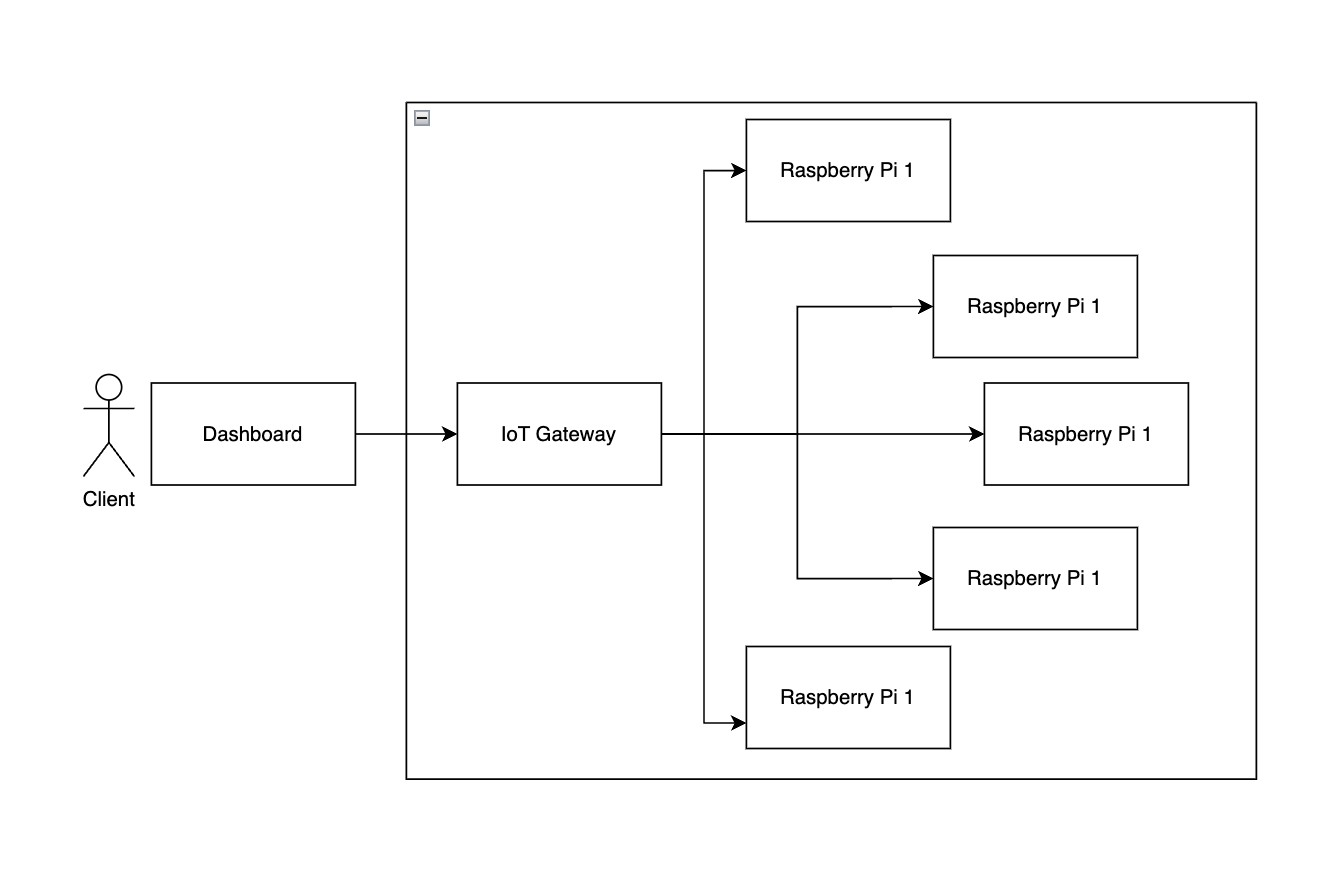
\includegraphics[width=0.5\textwidth]{resources/chapter-3/gambaran-umum-arsitektur.jpg}
  \caption{Gambaran umum arsitektur yang akan dibuat}
  \label{fig:gambaran-umum-arsitektur}
\end{figure}